\documentclass[12pt,utf8,notheorems,compress,t,aspectratio=169]{beamer}
\usepackage{etex}
\usepackage{pgfpages}
\usepackage{calc}
\usepackage[export]{adjustbox}
\usepackage[ngerman]{babel}
\usepackage[normalem]{ulem}
\usepackage{mathtools}
\usepackage{booktabs}
\usepackage{stmaryrd}
\usepackage{amssymb}
\usepackage{manfnt}
\usepackage{array}
\usepackage{ragged2e}
\usepackage{multicol}
\usepackage{tabto}
\usepackage{xstring}
\usepackage{xspace}
\usepackage{proof}
\usepackage[all]{xy}
\xyoption{rotate}
\usepackage{tikz}
\usetikzlibrary{tikzmark,decorations.pathreplacing,calc,shapes,shapes.callouts,shapes.arrows,patterns,fit,backgrounds,decorations.pathmorphing,positioning,svg.path}
\hypersetup{colorlinks=true}
\usepackage[protrusion=true,expansion=true]{microtype}
\usepackage{pifont}
\usepackage[skins]{tcolorbox}

\setbeamersize{text margin left=1.60em,text margin right=1.60em}

% from Dominik Kirst
\newtcolorbox{emptybox}{
  beamer,
  width=(0.68\textwidth),
  % enlarge left by=-3pt,
  titlerule=0mm,
  colframe=white,
  coltitle=black,
  bottom=6pt,
  top=-12pt,
  left=6pt,
  right=6pt,
  notitle,
  adjusted title={},
  outer arc=.5mm,
  arc=.5mm,
  no shadow,
  fuzzy shadow={1mm}{-1mm}{-1.2mm}{.7mm}{black!20},
  interior titled code={}
}

\newcommand{\cmark}{\ding{51}}
\newcommand{\xmark}{\ding{55}}
\DeclareSymbolFont{extraup}{U}{zavm}{m}{n}
\DeclareMathSymbol{\varheart}{\mathalpha}{extraup}{86}

\graphicspath{{images/}}

\setlength\parskip{\medskipamount}
\setlength\parindent{0pt}

\title{Das Auswahlaxiom: Fraktale Monster, Sandkästen und eine unerwartete Schlussfolgerung}

\author{Ingo Blechschmidt}
\date{3. Juni 2025}

%\setbeameroption{show notes on second screen=bottom}
\newcommand{\jnote}[2]{\only<#1>{\note{\usebackgroundtemplate{x}\setlength\parskip{\medskipamount}\footnotesize\justifying#2\par}}}
\setbeamertemplate{note page}[plain]

\useinnertheme{rectangles}

\usecolortheme{seahorse}
\definecolor{mypurple}{RGB}{253,73,34}
\definecolor{mypurpledark}{RGB}{100,0,150}
\setbeamercolor{structure}{fg=mypurple}
\setbeamercolor*{title}{bg=mypurple,fg=white}
\setbeamercolor*{titlelike}{bg=mypurple,fg=white}
\setbeamercolor{frame}{bg=black}
\setbeamertemplate{blocks}[rounded][shadow=true]

\usefonttheme{serif}
\usepackage[T1]{fontenc}
\usepackage{libertine}

\newcommand{\NN}{\mathbb{N}}
\newcommand{\RR}{\mathbb{R}}

\setbeamertemplate{frametitle}{%
  \leavevmode%
  \vskip-1.6em%
  \begin{beamercolorbox}[dp=1ex,center,wd=\paperwidth,ht=2.25ex]{title}%
    \vskip0.5em%
    \bf\insertframetitle
  \end{beamercolorbox}%

  \vskip-0.77em\hspace*{-2em}%
  \textcolor{mypurpledark}{\rule[0em]{1.1\paperwidth}{2.4pt}}

  \vskip-0.4em%
}

\setbeamertemplate{navigation symbols}{}

\newcommand{\insertframeextra}{}
\setbeamertemplate{footline}{%
  \begin{beamercolorbox}[wd=\paperwidth,ht=2.25ex,dp=1ex,right,rightskip=1mm,leftskip=1mm]{}%
    % \inserttitle
    \hfill
    \insertframenumber\insertframeextra\,/\,\inserttotalframenumber
  \end{beamercolorbox}%
  \vskip0pt%
}

\newcommand{\hil}[1]{{\usebeamercolor[fg]{item}{\textbf{#1}}}}
\newcommand{\bad}[1]{\textcolor{red!90}{\textnormal{#1}}}
\newcommand{\good}[1]{\textcolor{mypurple}{\textnormal{#1}}}

\newcommand{\normalnumber}[1]{%
  {\renewcommand{\insertenumlabel}{#1}\!\usebeamertemplate{enumerate item}\!}
}
\newcommand{\bignumber}[1]{%
  \renewcommand{\insertenumlabel}{#1}\scalebox{1.2}{\!\usebeamertemplate{enumerate item}\!}
}

\begin{document}

\addtocounter{framenumber}{-1}

{\usebackgroundtemplate{\begin{minipage}{\paperwidth}\centering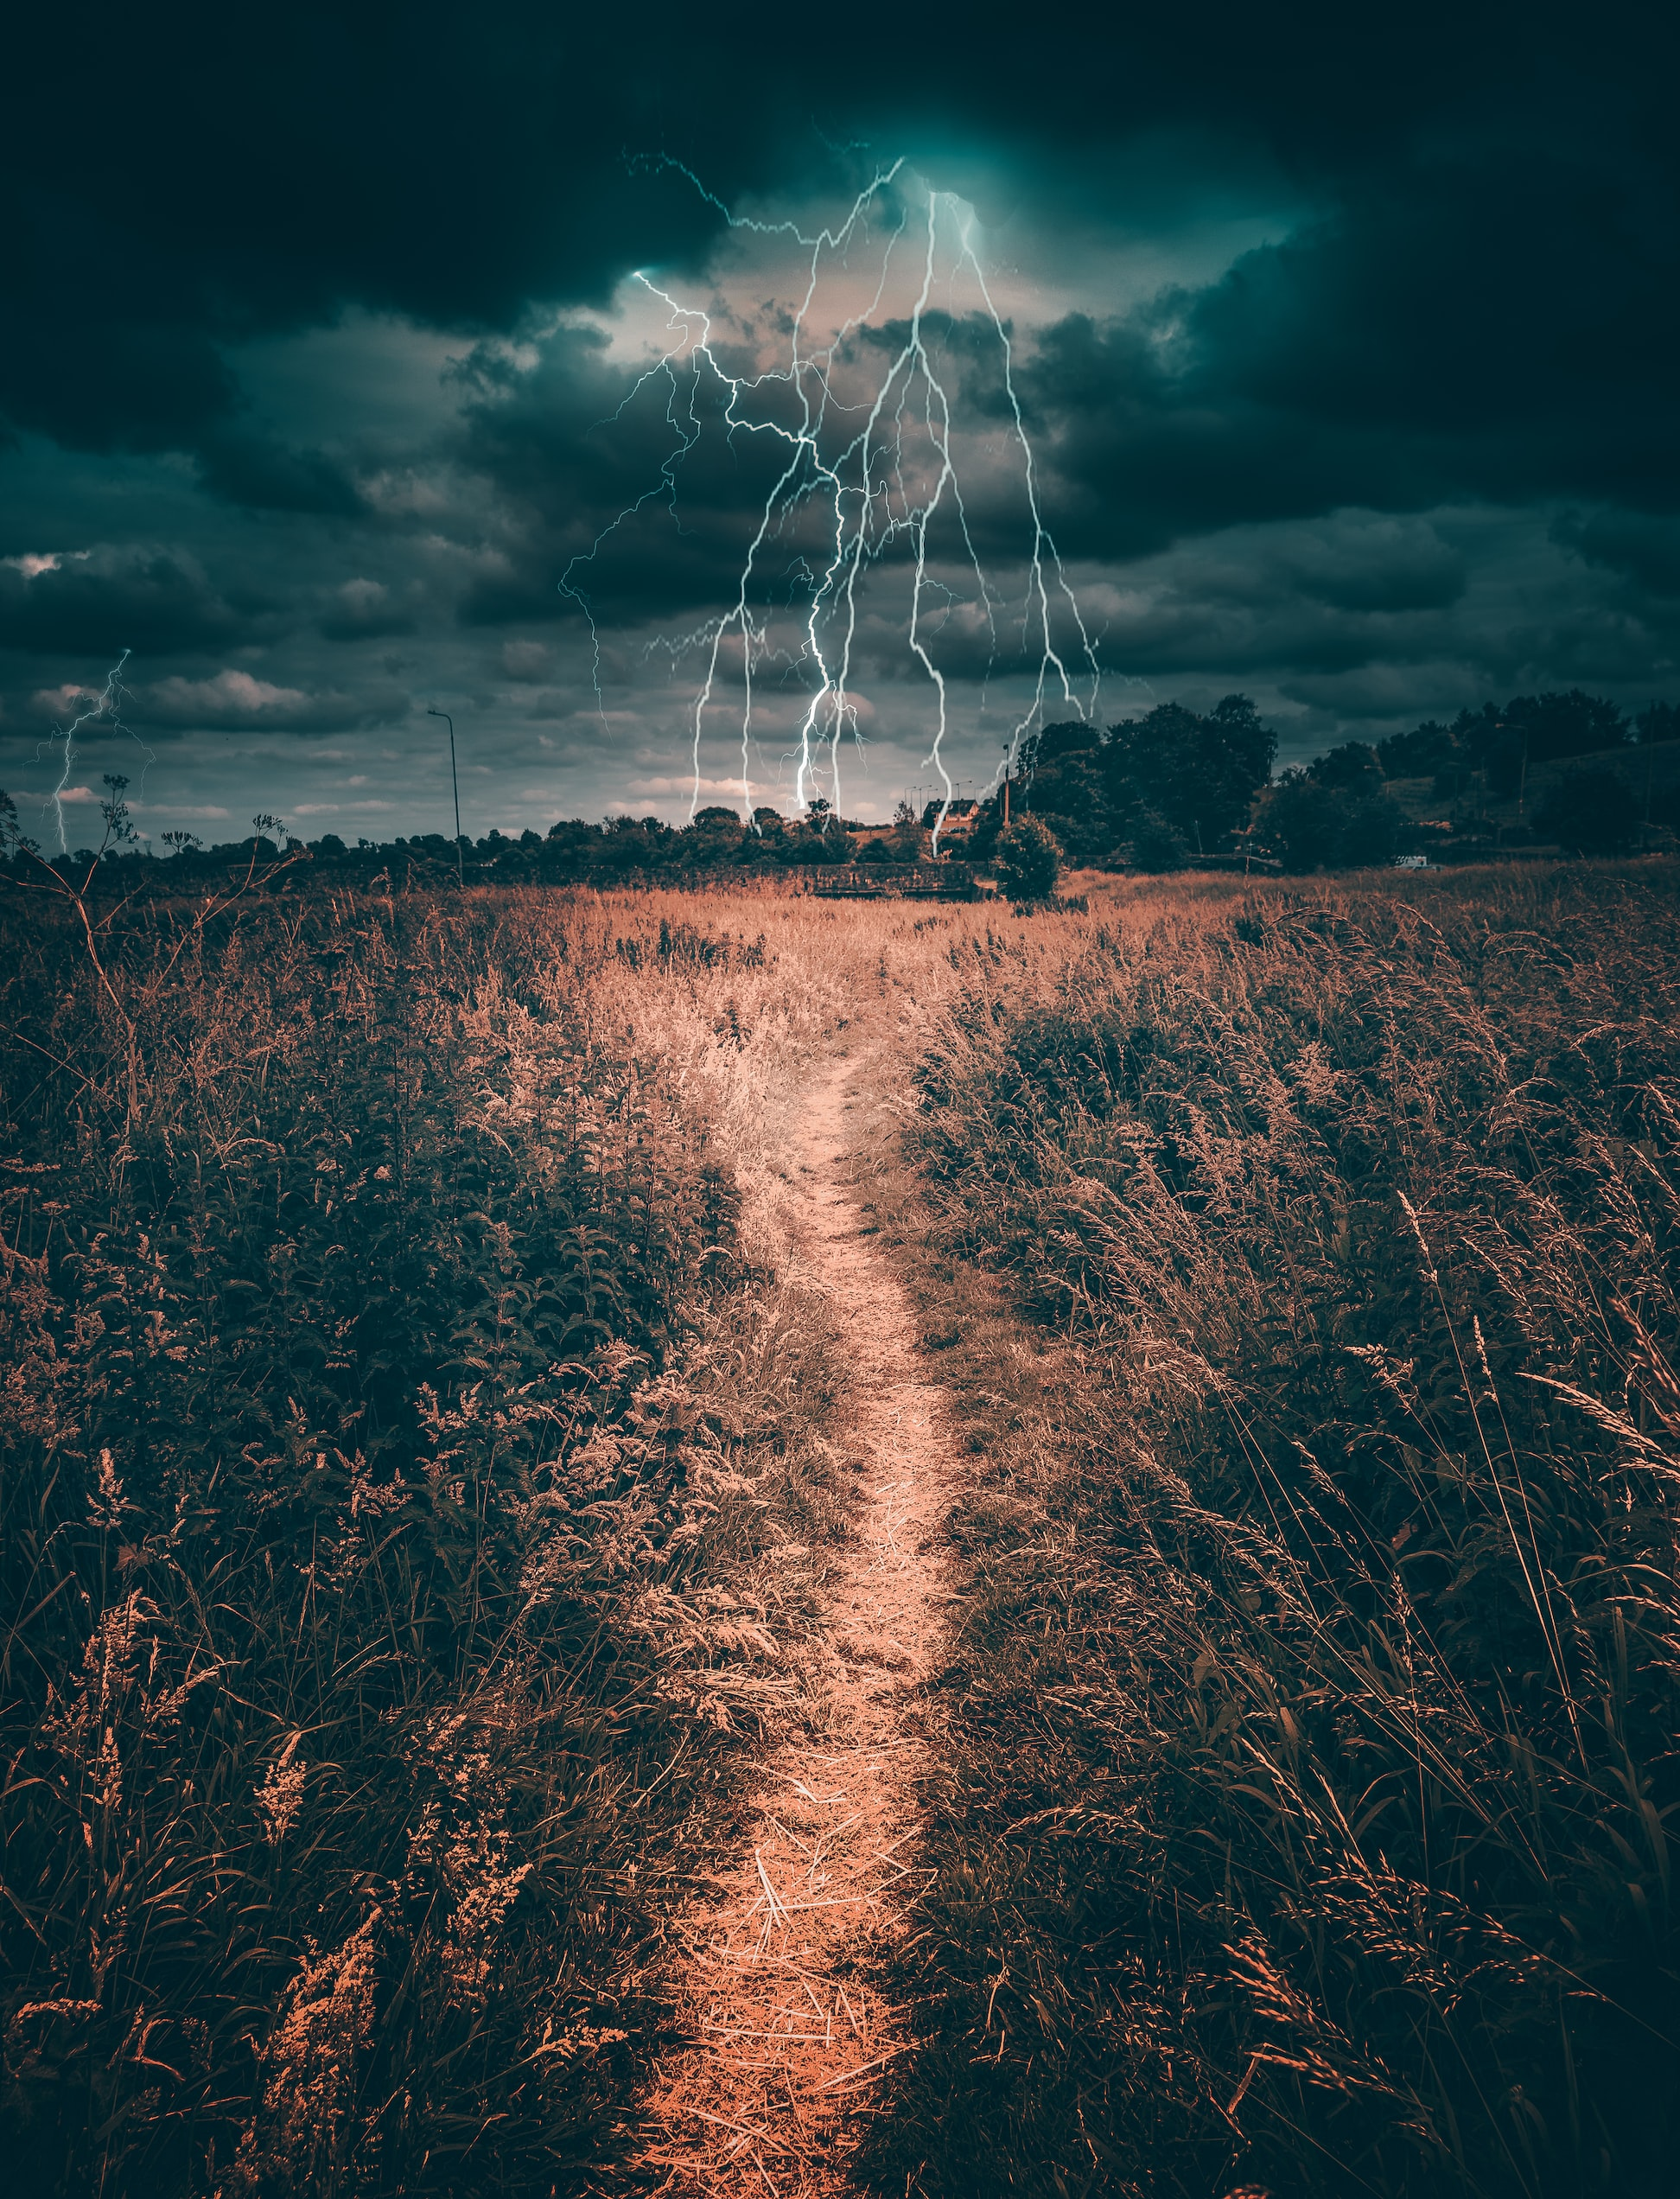
\includegraphics[width=\paperwidth]{lightning}\end{minipage}}
\begin{frame}[c]
  \centering

  \bigskip
  \bigskip
  \bigskip
  \bigskip

  \scriptsize

  \setbeamercolor{block body}{bg=black!100}
  \begin{minipage}{0.62\textwidth}
    \begin{block}{}
      \centering\normalsize\color{white}
      \hil{\phantom{g}Das Auswahlaxiom: Fraktale Monster, Sandkästen
      und eine unerwartete Schlussfolgerung\phantom{g}}
    \end{block}
  \end{minipage}

  \color{white}
  \textit{-- eine Einladung --}

  \vspace*{9.9em}
  \raisebox{0pt}[0pt][0pt]{\hspace*{-2.4em}\begin{minipage}[0em]{\paperwidth}\centering%
    \only<1>{
      Ingo Blechschmidt \medskip

      Seminar zur Philosophie der Mathematik \\
      3. Juni 2025
    }
    \only<2->{\href{https://www.spikedmath.com/}{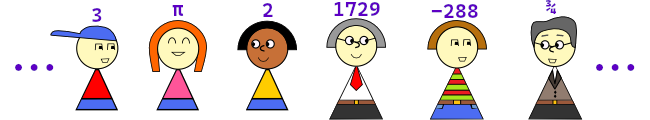
\includegraphics[width=\paperwidth]{long-queue}}}
  \end{minipage}}
\end{frame}}

\definecolor{mypurple}{RGB}{150,0,255}
\setbeamercolor{structure}{fg=mypurple}

{\usebackgroundtemplate{\begin{minipage}{\paperwidth}\centering
\includegraphics[width=\paperwidth]{lightning-lighter}\end{minipage}}
\begin{frame}{Auswahlfunktionen}
  \setbeamercolor{block body}{bg=white!100}
  {\centering\emph{\scriptsize Das Auswahlaxiom (\textsc{ac}) besagt:}\\[-0.5em]\begin{emptybox}
    \centering
    "`Für \hil{jedes} System bewohnter Mengen \\
    gibt es eine \hil{Auswahlfunktion}, die \\
    jeder dieser Mengen einen \hil{Repräsentanten} zuordnet."'
  \end{emptybox}\par}
  \bigskip
  \pause

  Beispiele für Funktionen:
  \vspace*{-0.2em}
  \begin{enumerate}
    \small
    \item Sinusfunktion: $x \mapsto \sin(x)$
    \item Quadrierungsfunktion: $x \mapsto x^2$, so $1 \mapsto 1,\ 2 \mapsto 4,\
    3 \mapsto 9,\ \ldots$
    \item \textsf{computeAreaOfCircle}: $r \mapsto \pi r^2$, so $1 \mapsto
    \pi,\ 2 \mapsto 4 \pi,\ \ldots$
    \pause
    \item \textsf{lookupMayorOfCity}\tikzmark{start}
    \item \textsf{getYoungestStudentOfClass}\tikzmark{end}
  \end{enumerate}

  \begin{tikzpicture}[remember picture,overlay]
    \draw[decorate,decoration={brace,raise=12pt}]
      ([yshift=2ex]{{pic cs:end}|-{pic cs:start}}) --
      node[xshift=15pt,anchor=west] {"`Auswahlfunktionen"' \qquad 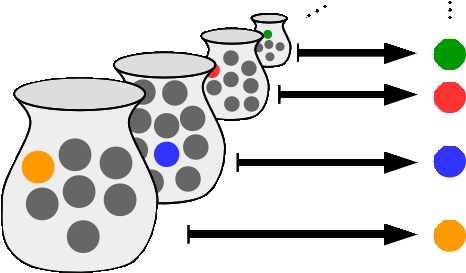
\includegraphics[valign=m,width=7em]{choice-function}}
      ([yshift=-0.5ex]pic cs:end);
  \end{tikzpicture}
  \vspace*{-1.5em}
  \pause

  \hil{Note.} Das Auswahlaxiom ist \hil{überflüssig} für \ldots
  \vspace*{-2em}
  \begin{columns}
    \small
    \begin{column}{0.28\textwidth}
      \begin{enumerate}
        \item[\bignumber{A}] \hil{endliche} Systeme bewohnter Mengen
      \end{enumerate}
    \end{column}
    \begin{column}{0.67\textwidth}
      \begin{enumerate}
        \item[\bignumber{B}] Systeme von bewohnten herauslösbaren Mengen natürlicher Zahlen
      \end{enumerate}
    \end{column}
  \end{columns}
\end{frame}}

\newcommand{\Fbox}[1]{{\color{gray!50}\fbox{\color{black}#1}}}
\newcommand{\konfig}[6]{
  \ldots
  \Fbox{\ensuremath{\stackrel{#1}{
\includegraphics[height=0.4em]{player-1}}}}\
  \Fbox{\ensuremath{\stackrel{#2}{
\includegraphics[height=0.4em]{player-2}}}}\
  \Fbox{\ensuremath{\stackrel{#3}{
\includegraphics[height=0.4em]{player-3}}}}\
  \Fbox{\ensuremath{\stackrel{#4}{
\includegraphics[height=0.4em]{player-4}}}}\
  \Fbox{\ensuremath{\stackrel{#5}{
\includegraphics[height=0.4em]{player-5}}}}\
  \Fbox{\ensuremath{\stackrel{#6}{
\includegraphics[height=0.4em]{player-6}}}}
  \ldots}

\begin{frame}{Aus Auswahlfunktion mach Gewinnstrategie}
  \small
  \hspace*{-0.35cm}\mbox{Für das System der \hil{Mengen nahezu-identischer Szenarien} könnte eine
  Auswahlfunktion sein:}
  \[
    \small
    \begin{array}{ccc}
      \left\{
        \begin{array}{c}
          \konfig{3}{3}{3}{3}{3}{3} \\
          \konfig{3}{3}{3}{1}{3}{3} \\
          \konfig{3}{3}{3}{1}{1}{3} \\
          \text{(und viele weitere Szenarien)}
        \end{array}
      \right\} &\longmapsto&
      \konfig{3}{3}{3}{3}{3}{3} \\
      \\[-1em]
      \left\{
        \begin{array}{c}
          \konfig{1}{2}{1}{2}{1}{2} \\
          \konfig{1}{2}{1}{4}{1}{2} \\
          \konfig{1}{2}{1}{5}{1}{2} \\
          \text{(und viele weitere Szenarien)}
        \end{array}
      \right\} &\longmapsto&
      \konfig{1}{2}{1}{2}{1}{2} \\
      \\[-1em]
      \text{(und viele weitere Mengen)} && \text{(und viele weitere Repräsentanten)}
    \end{array}
  \]

  \begin{columns}[c]
    \begin{column}{0.00\textwidth}
      \vspace*{0.5em}
\includegraphics[valign=m,height=1.0em]{lightbulb}
    \end{column}
    \begin{column}{0.9\textwidth}
      Wenn die Zwerge eine \hil{gemeinsame Auswahlfunktion} nutzen,
      um ihre Vermutungen abzugeben, werden nur \hil{endlich viele}
      falsch liegen.
    \end{column}
  \end{columns}
\end{frame}

\begin{frame}{Folgerungen aus dem Auswahlaxiom}
  \centering
  \hil{"`Seltsame"':}
  \medskip
  \begin{columns}
    \begin{column}{0.2\textwidth}
      \centering
      \href{https://infinityplusonemath.wordpress.com/2017/10/31/non-measurable-sets-that-go-bump-in-the-night/}{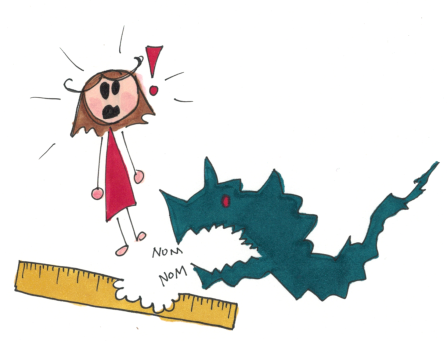
\includegraphics[height=4em]{non-measurable-monster}} \\
      Vitali-Fraktal
    \end{column}
    \begin{column}{0.6\textwidth}
      \centering
      \href{https://en.wikipedia.org/wiki/Banach\%E2\%80\%93Tarski_paradox}{
\includegraphics[height=4em]{banach-tarski}}
      Banach--Tarski-Paradoxon
    \end{column}
    \begin{column}{0.15\textwidth}
      \centering
      \href{https://mathoverflow.net/questions/151286/probabilities-in-a-riddle-involving-axiom-of-choice}{
\includegraphics[height=4em]{crystal-ball}}
      Weissagung
    \end{column}
  \end{columns}
  \bigskip
  \bigskip

  \hil{"`Gut/prokrastinatorisch"':}
  \medskip
  \begin{columns}
    \begin{column}{0.55\textwidth}
      \centering
      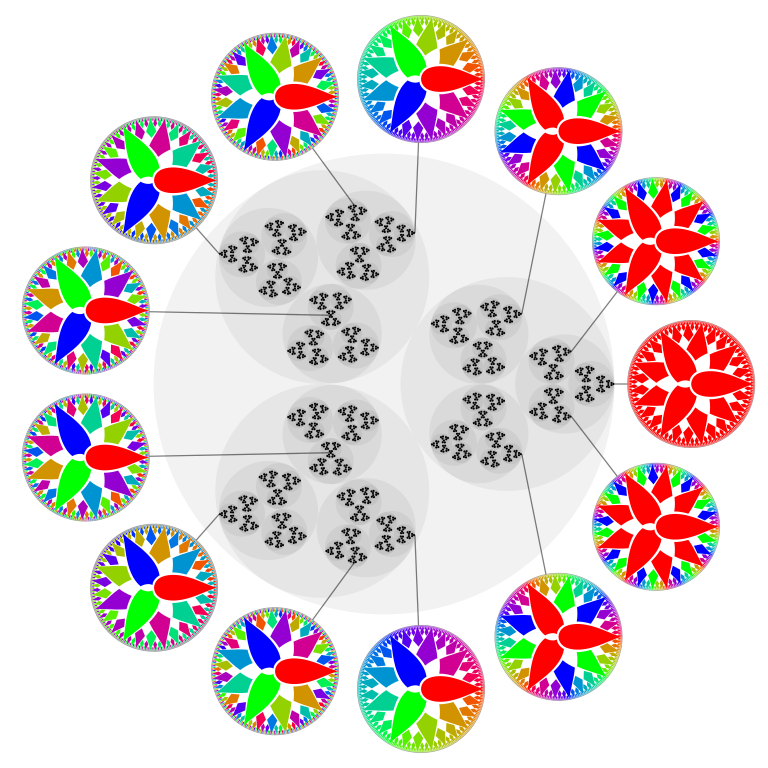
\includegraphics[height=4em]{p-adic} \\
      Jeder Körper hat einen algebraischen Abschluss.
    \end{column}
    \begin{column}{0.4\textwidth}
      \centering
      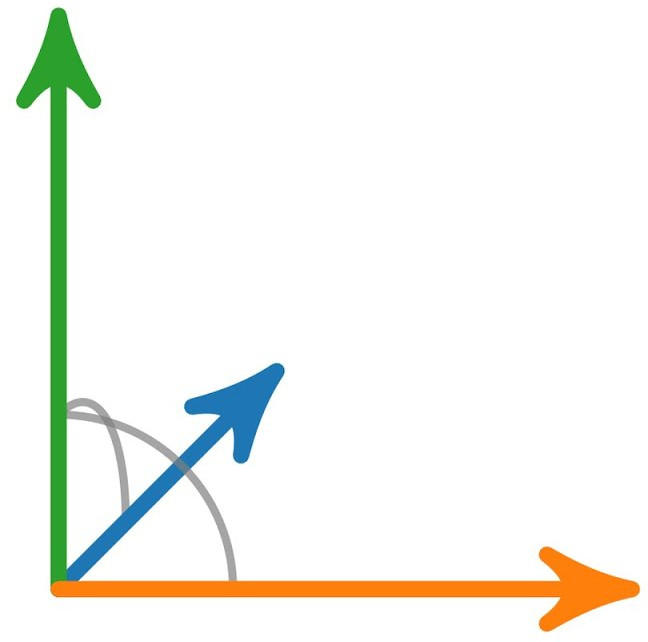
\includegraphics[height=4em]{basis} \\
      Jeder Vektorraum hat eine Basis.
    \end{column}
  \end{columns}
\end{frame}

\newcommand{\expl}[2]{
  \justifying
  "`$\text{\normalnumber{#1}}$"' im effektiven Topos bedeutet: #2
}
\newcommand{\qswitch}[3]{\only<1-#1>{
\includegraphics[height=0.7em]{question-mark}}\only<#2->{#3}}
\newcommand{\ccmark}{\good{\cmark}}
\newcommand{\cxmark}{\bad{\xmark}}
\newcommand{\notnot}{\emph{nicht~nicht}\xspace}
\begin{frame}{Ein Alternativuniversum: der effektive Topos}
  \centering
  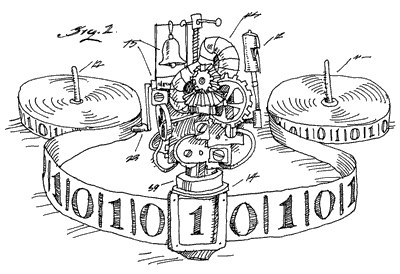
\includegraphics[width=6.5em]{turing-machine}
  \small

  \begin{tabular}{@{\!\!\!\!\!\!}l@{\,}p{9cm}lp{1.8cm}}
    \toprule
    & Aussage & in $\mathsf{Set}$ & in $\mathsf{Eff}$ \\
    \midrule
    \normalnumber{1} & Jede Zahl ist prim oder nicht prim. & \ccmark{}
    (trivial) & \ccmark \\
    \normalnumber{2} & Nach jeder Zahl kommt eine Primzahl. & \ccmark & \ccmark \\
    \normalnumber{3} & Jede Abbildung $\NN \to \NN$ hat eine Nullstelle oder nicht. & \ccmark{} (trivial) & \cxmark \\
    \normalnumber{4} & Jede Abbildung $\NN \to \NN$ ist berechenbar. & \cxmark &
    \qswitch{4}{5}{\ccmark}\only<1-4>{\,} \visible<5->{(trivial)} \\
    \normalnumber{5} & Jede Abbildung $\RR \to \RR$ ist stetig. & \cxmark &
    \qswitch{5}{6}{\ccmark{} (falls MP)} \\
    \normalnumber{6} & Jede Abbildung $\NN \to \NN$, die \notnot{} eine
    Nullstelle hat, hat eine Nullstelle. & \ccmark{} (trivial) &
    \qswitch{6}{7}{\ccmark{} (falls MP)} \\
    %\normalnumber{7} & Countable choice holds. & \ccmark &
    %\qswitch{7}{8}{\ccmark{} (always!)} \\
    %\normalnumber{8} & Heyting-Arithmetik ist kategorisch. & \cxmark &
    %\qswitch{8}{9}{\ccmark{} (falls MP)} \\
    %\normalnumber{9} & A statement holds iff it is realized. & \cxmark &
    %\qswitch{9}{10}{\ccmark} \\
    \bottomrule
  \end{tabular}
  \medskip

  \only<1>{\color{white}Es gibt eine Maschine, die von einer beliebigen Zahl
  bestimmt, ob sie prim ist oder nicht. \\\ \\\ }
  \only<2>{\expl{1}{Es gibt eine Maschine, die von einer beliebigen Zahl
  bestimmt, ob sie prim ist oder nicht. \\\ \\\ }}
  \only<3>{\expl{2}{Es gibt eine Maschine, die eine beliebige Zahl~$n$
  einliest und eine Primzahl größer als~$n$ ausgibt. \\\ \\\ }}
  \only<4>{\expl{3}{Es gibt eine Maschine, die eine beliebige Maschine einliest,
  die eine Funktion~$f : \NN \to \NN$ berechnet, und bestimmt, ob~$f$ eine
  Nullstelle hat oder nicht. \\\ \\\ }}
  \only<5>{\expl{4}{Es gibt eine Maschine, die eine beliebige Maschine
  einliest, die eine Funktion~$f : \NN \to \NN$ berechnet, und eine Maschine
  ausgibt, die~$f$ berechnet. \hfill \emph{cat!} \\\ \\\ }}
  \only<7>{\expl{6}{Es gibt eine Maschine, die eine beliebige Maschine,
  die eine Funktion~$f : \NN \to \NN$ berechnet, sowie ein bloßes Versprechen,
  dass es \notnot nicht der Fall ist, dass~$f$ eine Nullstelle hat, einliest,
  und eine Nullstelle von~$f$ bestimmt.
  \hfill \emph{unbeschränkte Suche!}}}
  %\only<8>{\expl{7}{\justifying There is a machine which, given a machine
  %computing for every~$x \in \NN$ some~$y \in A$ together with a realizer
  %of~$\varphi(x,y)$, outputs a machine computing a suitable choice
  %function~$\NN \to A$.}}
  %\only<9>{\ \\\ \\\ \\\ }
  \bigskip
  \pause
  \pause
  \pause
  \pause
  \pause
  \pause
  \pause

  \begin{columns}
    \begin{column}{0.00\textwidth}
      \dbend
    \end{column}
    \begin{column}{0.9\textwidth}
      In $\mathsf{Eff}$ gibt es \hil{keine} Auswahlfunktion für das System
      der \\ \hil{Mengen verhaltensgleicher Programme}.
    \end{column}
  \end{columns}
\end{frame}

\begin{frame}{Ein Gegenbeispiel zum Auswahlaxiom}
  Eine \hil{Auswahlfunktion} für das System der
  \hil{Mengen verhaltensgleicher Programme} könnte so aussehen:
  \[
    \small
    \begin{array}{lll}
      \left\{
        \begin{array}{l}
          \textsf{while True: pass} \\
          \textsf{while 2 == 1 + 1: pass} \\
          \textsf{s = 'a'; while len(s) > 0: s = s + 'a'} \\
          \vdots
        \end{array}
      \right\} &\longmapsto&
      \textsf{while True: pass} \\
      \\[-0.5em]
      \left\{
        \begin{array}{l}
          \textsf{print(2+2)} \\
          \textsf{print(4)} \\
          \textsf{print(len('37c3'))} \\
          \vdots
        \end{array}
      \right\} &\longmapsto&
      \textsf{print(4)} \\
      \\[-0.6em]
      \vdots && \vdots
    \end{array}
  \]

  Mit solch einer Auswahlfunktion~\textsf{c} ließe sich ein \hil{Halteorakel}
  bauen: \\
  Ein Programm~$p$ divergiert genau dann, wenn~$\textsf{c}(p) = \textsf{c}(\textsf{'while True: pass'})$.
\end{frame}

\newcommand{\Fboxs}[1]{\Fbox{\begin{minipage}[c][2em]{2em}\centering\ensuremath{#1}\end{minipage}}}
\begin{frame}{Eine nuancierte Perspektive}
  \begin{enumerate}
    \item Es gibt ein Gegen-Axiom, das \hil{Determiniertheitsaxiom}
    (\textsc{ad}): \\
    "`Jede Instanz des \hil{Folgenspiels} ist \hil{determiniert}."'

    {\small\justifying
    Wie auch bei \textsc{ac} folgt die finitäre Version von \textsc{ad} aus unbestrittenen
    grundlegenden Axiomen.
    \emph{\textsc{ac} und \textsc{ad} sind zwei verschiedene
    Extrapolierungen des Endlichen ins Unendliche.}\par}
    \bigskip
    \vspace*{-0.1em}
    \pause

    \item\justifying Das Auswahlaxiom zieht definitiv \hil{keine neuen}
    Inkonsistenzen mit sich
    (falls~\textsc{zfc} inkonsistent sein sollte, so auch~\textsc{zf} --
    bewiesenermaßen in~\textsc{ipra}).

    {\small\emph{Befürchtungen über Inkonsistenz des Auswahlaxioms sind
    folglich unbegründet.}}
    \bigskip
    \vspace*{-0.1em}
    \pause

    \item Sogar falls \textsc{ac} in der Metatheorie nicht verfügbar ist,
    gilt \textsc{ac} immer noch in~$L$, \hil{Gödels Sandbox}.
    Wunderbarerweise haben \textsf{Set} und $L$ dasselbe~$\NN$.
    Daher gelten in \textsf{Set} und $L$ dieselben arithmetischen Wahrheiten.
    Von jedem ZFC-Beweis einer solchen Wahrheit lässt sich \textsc{ac}
    \hil{maschinell eliminieren}.

    {\small\emph{Das Auswahlaxiom kann dadurch als \hil{nützliche Fiktion}
    betrachtet werden, ähnlich wie negative Zahlen nützlich sind, aber man auch
    damit vorlieb nehmen könnte, separat Guthaben und Schulden aufzuführen.
    Das Auswahlaxiom wird für gewisse infrastrukturelle Werkzeuge benötigt,
    ist aber für arithmetische Konsequenzen dieser Werkzeuge überflüssig}.\par}
    \bigskip
  \end{enumerate}
\end{frame}

\addtocounter{framenumber}{-1}
\begin{frame}[plain]
  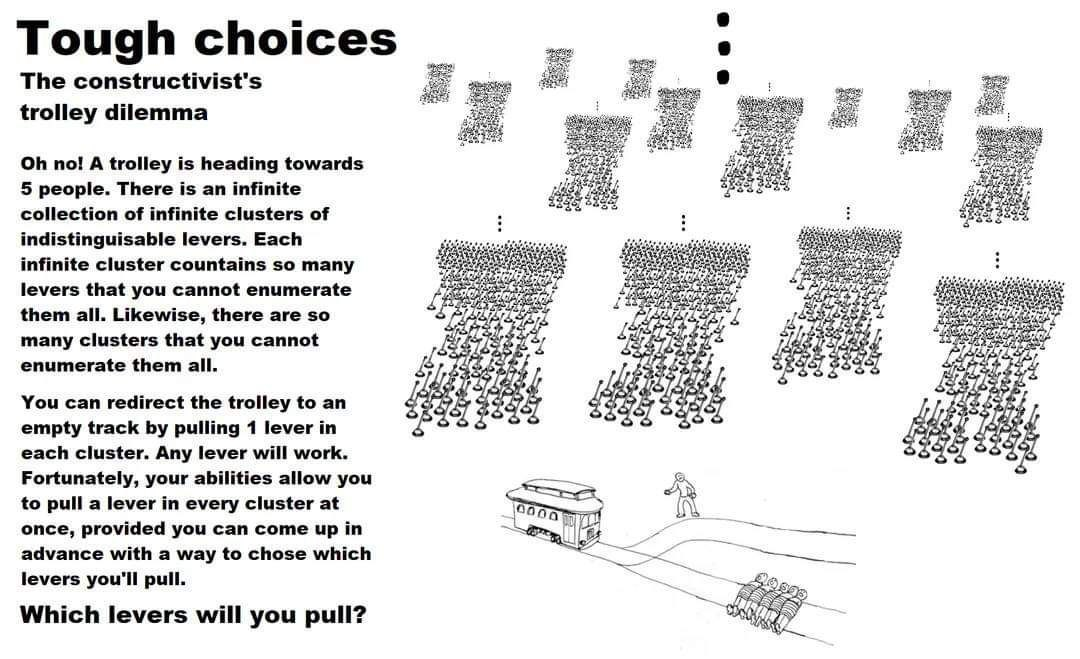
\includegraphics[width=\textwidth]{tough-choices}
\end{frame}

\end{document}

Ideas for a more specifically mathematical audience:
- Slide on what AC is not
- Slide on DC
